\documentclass[11pt,french,french]{article}
\usepackage{lmodern}
\usepackage{amssymb,amsmath}
\usepackage{ifxetex,ifluatex}
\usepackage{fixltx2e} % provides \textsubscript
\ifnum 0\ifxetex 1\fi\ifluatex 1\fi=0 % if pdftex
  \usepackage[T1]{fontenc}
  \usepackage[utf8]{inputenc}
\else % if luatex or xelatex
  \ifxetex
    \usepackage{mathspec}
    \usepackage{xltxtra,xunicode}
  \else
    \usepackage{fontspec}
  \fi
  \defaultfontfeatures{Mapping=tex-text,Scale=MatchLowercase}
  \newcommand{\euro}{€}
\fi
% use upquote if available, for straight quotes in verbatim environments
\IfFileExists{upquote.sty}{\usepackage{upquote}}{}
% use microtype if available
\IfFileExists{microtype.sty}{%
\usepackage{microtype}
\UseMicrotypeSet[protrusion]{basicmath} % disable protrusion for tt fonts
}{}
\usepackage[margin=1in]{geometry}
\ifxetex
  \usepackage{polyglossia}
  \setmainlanguage{}
\else
  \usepackage[shorthands=off,french]{babel}
\fi
\usepackage{color}
\usepackage{fancyvrb}
\newcommand{\VerbBar}{|}
\newcommand{\VERB}{\Verb[commandchars=\\\{\}]}
\DefineVerbatimEnvironment{Highlighting}{Verbatim}{commandchars=\\\{\}}
% Add ',fontsize=\small' for more characters per line
\usepackage{framed}
\definecolor{shadecolor}{RGB}{248,248,248}
\newenvironment{Shaded}{\begin{snugshade}}{\end{snugshade}}
\newcommand{\AlertTok}[1]{\textcolor[rgb]{0.94,0.16,0.16}{#1}}
\newcommand{\AnnotationTok}[1]{\textcolor[rgb]{0.56,0.35,0.01}{\textbf{\textit{#1}}}}
\newcommand{\AttributeTok}[1]{\textcolor[rgb]{0.77,0.63,0.00}{#1}}
\newcommand{\BaseNTok}[1]{\textcolor[rgb]{0.00,0.00,0.81}{#1}}
\newcommand{\BuiltInTok}[1]{#1}
\newcommand{\CharTok}[1]{\textcolor[rgb]{0.31,0.60,0.02}{#1}}
\newcommand{\CommentTok}[1]{\textcolor[rgb]{0.56,0.35,0.01}{\textit{#1}}}
\newcommand{\CommentVarTok}[1]{\textcolor[rgb]{0.56,0.35,0.01}{\textbf{\textit{#1}}}}
\newcommand{\ConstantTok}[1]{\textcolor[rgb]{0.00,0.00,0.00}{#1}}
\newcommand{\ControlFlowTok}[1]{\textcolor[rgb]{0.13,0.29,0.53}{\textbf{#1}}}
\newcommand{\DataTypeTok}[1]{\textcolor[rgb]{0.13,0.29,0.53}{#1}}
\newcommand{\DecValTok}[1]{\textcolor[rgb]{0.00,0.00,0.81}{#1}}
\newcommand{\DocumentationTok}[1]{\textcolor[rgb]{0.56,0.35,0.01}{\textbf{\textit{#1}}}}
\newcommand{\ErrorTok}[1]{\textcolor[rgb]{0.64,0.00,0.00}{\textbf{#1}}}
\newcommand{\ExtensionTok}[1]{#1}
\newcommand{\FloatTok}[1]{\textcolor[rgb]{0.00,0.00,0.81}{#1}}
\newcommand{\FunctionTok}[1]{\textcolor[rgb]{0.00,0.00,0.00}{#1}}
\newcommand{\ImportTok}[1]{#1}
\newcommand{\InformationTok}[1]{\textcolor[rgb]{0.56,0.35,0.01}{\textbf{\textit{#1}}}}
\newcommand{\KeywordTok}[1]{\textcolor[rgb]{0.13,0.29,0.53}{\textbf{#1}}}
\newcommand{\NormalTok}[1]{#1}
\newcommand{\OperatorTok}[1]{\textcolor[rgb]{0.81,0.36,0.00}{\textbf{#1}}}
\newcommand{\OtherTok}[1]{\textcolor[rgb]{0.56,0.35,0.01}{#1}}
\newcommand{\PreprocessorTok}[1]{\textcolor[rgb]{0.56,0.35,0.01}{\textit{#1}}}
\newcommand{\RegionMarkerTok}[1]{#1}
\newcommand{\SpecialCharTok}[1]{\textcolor[rgb]{0.00,0.00,0.00}{#1}}
\newcommand{\SpecialStringTok}[1]{\textcolor[rgb]{0.31,0.60,0.02}{#1}}
\newcommand{\StringTok}[1]{\textcolor[rgb]{0.31,0.60,0.02}{#1}}
\newcommand{\VariableTok}[1]{\textcolor[rgb]{0.00,0.00,0.00}{#1}}
\newcommand{\VerbatimStringTok}[1]{\textcolor[rgb]{0.31,0.60,0.02}{#1}}
\newcommand{\WarningTok}[1]{\textcolor[rgb]{0.56,0.35,0.01}{\textbf{\textit{#1}}}}
\ifxetex
  \usepackage[setpagesize=false, % page size defined by xetex
              unicode=false, % unicode breaks when used with xetex
              xetex]{hyperref}
\else
  \usepackage[unicode=true]{hyperref}
\fi
\hypersetup{breaklinks=true,
            bookmarks=true,
            pdfauthor={},
            pdftitle={},
            colorlinks=true,
            citecolor=blue,
            urlcolor=blue,
            linkcolor=magenta,
            pdfborder={0 0 0}}
\urlstyle{same}  % don't use monospace font for urls
\setlength{\parindent}{0pt}
\setlength{\parskip}{6pt plus 2pt minus 1pt}
\setlength{\emergencystretch}{3em}  % prevent overfull lines
\setcounter{secnumdepth}{5}

%%% Use protect on footnotes to avoid problems with footnotes in titles
\let\rmarkdownfootnote\footnote%
\def\footnote{\protect\rmarkdownfootnote}


  \title{Analyse statistique et empirique des modèles\\
de Word Embedding sur Twitter}
    \author{Kim Antunez, Romain Lesauvage, Alain Quartier-la-Tente\\
sous l'encadrement de Benjamin Muller (Inria)}
    \date{}
  
\usepackage{caption}
\usepackage{graphicx}
\usepackage{natbib}

\begin{document}

\maketitle


\hypertarget{contexte}{%
\section{Contexte}\label{contexte}}

Grâce à l'évolution des méthodes d'apprentissage profond (\emph{Deep
Learning}), l'appréhension du langage naturel est aujourd'hui devenu une
discipline à part entière (\emph{Natural Language Processing}). Ce
succès s'explique en partie grâce à l'émergence de techniques non
supervisée d'apprentissage de représentation de structures
linguistiques. Les méthodes de \emph{word embedding} (« plongement
lexical » en français) permettent de représenter chaque mot d'un
dictionnaire par un vecteur de nombres réels afin que les mots qui
apparaissant dans des contextes similaires possèdent des vecteurs
correspondants qui sont relativement proches. Les modèles
\textbf{word2vec}, développés par une équipe de recherche chez Google
(\cite{Mikolov}), sont parmi les plus célèbres et sont ceux sur lesquels
se concentrera notre projet.

\hypertarget{objectif-du-projet}{%
\section{Objectif du projet}\label{objectif-du-projet}}

Dans ce projet de statistiques appliquées, nous étudierons dans un
premier temps en détail et implémenterons le modèle \emph{word2vec}.
Dans un second temps, nous appliquerons ce modèle sur une base de
données composée de plusieurs millions de tweets publiés en France entre
2013 et 2017. Pour ce faire, nous mobiliserons des techniques d'analyse
de sentiments afin de créer des indicateurs qui pourront être comparés
aux indicateurs produits dans la statistique publique, en particulier
concernant l'opinion des ménages.

\hypertarget{travail-effectuuxe9-jusqualors}{%
\section{Travail effectué
jusqu'alors}\label{travail-effectuuxe9-jusqualors}}

\hypertarget{appropriation-du-moduxe8le}{%
\subsection{Appropriation du modèle}\label{appropriation-du-moduxe8le}}

Pour débuter ce projet, nous nous sommes documentés sur les méthodes de
NLP et de Deep-learning en lisant la bibliographie ainsi que des
articles de blogs, en particulier concernant l'implémentation sur Python
du modèle. Ces différentes lectures nous ont permis de bien comprendre
les différentes étapes de l'algorithme dont l'objectif est, pour rappel,
de représenter les mots d'un corpus sous la forme d'un vecteur de nombre
réels. Différentes architectures du modèle word2vec existent ; nous nous
intéresserons ici à l'approche appelée \emph{Skip-gram}. À l'inverse de
l'approche \emph{Continuous bags of words}, le principe de
\emph{Skip-gram} est de prédire, pour chaque mot du vocabulaire, sa
probabilité d'être proche d'un mot appelé \emph{focus}.

Nous entraînons le modèle grâce à un algorithme qui peut se résumer à
ces quelques étapes :

\begin{itemize}
\item
  Nous partons de deux matrices de poids : une en entrée et une en
  sortie. La taille de ces matrices est fixée par le nombre de mots
  différents (vocabulaire) présents dans le corpus (lignes) et la
  dimension souhaitée des vecteurs en sortie (colonnes).
\item
  L'algorithme parcourt ensuite chaque phrase du corpus. Pour chaque
  phrase, un mot appelé \emph{focus} est sélectionné au hasard. Puis, on
  associe à chaque mot focus un mot \emph{contexte} tiré lui aussi au
  hasard dans une fenêtre autour du mot focus choisi.
\item
  Nous sélectionnons ensuite la ligne de la matrice en entrée
  correspondant au mot focus. En multipliant matriciellement cette ligne
  avec la matrice de sortie, nous obtenons un score (produit scalaire)
  qui mesure pour chaque mot du vocabulaire la probabilité d'appartenir
  au contexte du mot focus. Ce score est ensuite transformé en
  probabilité d'appartenance grâce à la fonction \emph{softmax}. Nous
  mettons ensuite à jour la fonction de perte (\emph{loss}) qui dépend
  de ce score.
\item
  Les matrices d'entrée et de sortie sont mises à jour successivement
  par descente de gradient
  \(\theta^{(t+1)} = \theta^{(t)} - \eta \nabla_\theta L(\theta^{(t)})\)
  avec \(\theta\) la matrice (entrée ou sortie), \(L(\theta)\) la
  fonction de perte et \(\eta\) le taux d'apprentissage (constante).
\item
  Ces étapes sont répétées pour l'ensemble des couples {[}focus,
  contexte{]}. Puis, l'ensemble de l'opération est répétée un certain
  nombre d'\emph{epochs} fixé au préalable .
\end{itemize}

Au fur et à mesure de l'apprentissage, les deux matrices d'entrée et
sortie sont actualisées, et de plus en plus pertinentes. À la fin de
l'algorithme, nous faisons la moyenne de ces matrices. C'est cette
moyenne qui représentera les vecteurs finaux de représentation des mots
du corpus.

\hypertarget{impluxe9mentation-du-moduxe8le}{%
\subsection{Implémentation du
modèle}\label{impluxe9mentation-du-moduxe8le}}

Après s'être approprié le fonctionnement du modèle \textbf{word2vec},
nous avons tous les trois implémenté individuellement le modèle sur
Python en utilisant la librairie Pytorch. Ce travail individuel a permis
à chacun d'approfondir la compréhension du modèle et d'obtenir une
version actuelle conforme aux recommandations de l'article de Mikolov.

En première étape, nous avons implémenté une version simplifiée du
modèle \emph{word2vec} en utilisant la fonction \emph{softmax} décrite
plus haut. Cette méthode est gourmande computationnellement puisqu'elle
nécessite d'actualiser à chaque étape l'intégralité des matrices.

C'est pourquoi nous avons en seconde étape implémenté une version plus
élaborée du modèle grâce à la méthode du \emph{negative sampling}. Cette
méthode est d'une part moins coûteuse en temps de calcul puisqu'elle
permet d'actualiser uniquement une partie de la matrice de poids (celle
qui concerne le mot contexte sur lequel on travaille). Elle permet
d'autre part de corriger la sur-estimation des poids des mots contextes
tirés au hasard puisqu'elle implique de tirer également au hasard des
mots qui ne sont pas dans le contexte du mot focus, mots pour lesquels
on va chercher à minimiser leur proximité au mot focus dans la fonction
de \emph{loss}.

\hypertarget{uxe9valuation-du-moduxe8le-impluxe9mentuxe9}{%
\subsection{Évaluation du modèle
implémenté}\label{uxe9valuation-du-moduxe8le-impluxe9mentuxe9}}

Malgré leurs utilisations presque généralisées, très peu de travaux
théoriques expliquent ce qui est réellement capturé par ces
représentations de mots. C'est pourquoi l'évaluation de l'efficacité de
ce modèle ne peut se faire qu'à l'aide de méthodes empiriques.

Avant de s'attaquer à notre jeu de données complet, nous avons effectué
une première évaluation sur un corpus fictif. Ce corpus est composé de
dix couples ({[}grand, petit{]}), associés à dix mots contexte
différents ({[}taille, géant, \ldots{}{]}). Nous avons ensuite formé un
corpus fictif de 10 000 phrases en tirant aléatoirement, pour chaque
phrase, un mot d'un couple, cinq mots du contexte et trois mots bruits.

Nous avons retenu à ce stade trois méthodes pour évaluer les vecteurs
obtenus en sortie du modèle :

\begin{itemize}
\item
  La \emph{similarité cosinus}, qui consiste à calculer le cosinus de
  l'angle entre deux vecteurs. Le cosinus vaudra alors 1 pour deux
  vecteurs identiques, -1 pour deux vecteurs opposés et 0 pour deux
  vecteurs indépendants.
\item
  Une \emph{analyse en composantes principales} (\emph{ACP}) qui
  consiste à projeter les vecteurs de mots sur un plus faible nombre
  d'axes afin de rendre l'information moins redondante et plus visuelle.
\item
  L'algorithme \emph{T-SNE}, ou \emph{t-distributed Stochastic Neighbor
  Embedding}, une autre technique de réduction de dimension, plus
  efficace que l'ACP dans le cas d'un nombre important de données.
  L'algorithme se fonde cette fois-ci sur une interprétation
  probabiliste des proximités et est non-linéaire.
\end{itemize}

Nous avons donc mis en oeuvre ces trois techniques sur notre corpus
fictif. Les résultats semblent concluants : la similarité cosinus montre
bien une forte corrélation entre les mots focus et contexte du corpus
initial et l'ACP et l'algorithme t-SNE permettent également de montrer
graphiquement cette proximité (cf.~figure \ref{fig:figure_evaluation}).

\footnotesize

\begin{Shaded}
\begin{Highlighting}[]
\NormalTok{mot_plus_proche(}\StringTok{"grand"}\NormalTok{, n }\OperatorTok{=} \DecValTok{50}\NormalTok{)}
\CommentTok{#[('énorme', 0.9914256427481623),}
\CommentTok{# ('taille', 0.9905528713008166),}
\CommentTok{# […]}
\CommentTok{# ('vanille', 0.06068283530950071),}
\CommentTok{# ('salissures', 0.0539210063101789)]}
\end{Highlighting}
\end{Shaded}

\normalsize

\hypertarget{perspectives}{%
\section{Perspectives}\label{perspectives}}

\hypertarget{impluxe9mentation-et-uxe9valuation}{%
\subsection{Implémentation et
évaluation}\label{impluxe9mentation-et-uxe9valuation}}

Nous travaillons actuellement à la mise en commun de nos implémentations
individuelles du modèle afin d'aboutir à une version finalisée du
modèle. Nous devrons ensuite faire tourner notre modèle sur les tweets
mis à notre disposition. Cette étape sera également l'occasion
d'optimiser les étapes chronophages du code si nécessaire.

Les vecteurs ainsi obtenus à l'issue de l'algorithme nous permettront
ensuite de procéder à l'évaluation du modèle sur données réelles. Pour
ce faire, en plus d'utiliser les données d'évaluation décrites
ci-dessus, nous mobiliserons une base de donnée qui demande à des
personnes d'indiquer si selon eux certains couples de mots sont proches
ou éloignés (\emph{Human Judgement Agreement}). Il faudra comparer cette
similarité subjective aux résultats de notre modèle. Cette comparaison
s'effectue grâce au calcul d'une \emph{corrélation de Spearman}.

\hypertarget{analyse}{%
\subsection{Analyse}\label{analyse}}

Notre objectif final est d'effectuer un travail d'analyse autour de la
comparaison entre les données produites par la statistique publique et
ce qu'il est possible d'obtenir grâce aux tweets. Différents échanges
avec l'Insee nous amènent à nous diriger vers une de ces différentes
problématiques :

\begin{itemize}
\item
  Les tweets permettent-ils d'obtenir des indicateurs synthétiques
  d'opinion des ménage proches de ceux produits dans la statistique
  publique (comme l'enquête de conjoncture Camme auprès des ménages,
  Insee) ?
\item
  Est-il possible de prévoir (géographiquement, temporellement) le taux
  de chômage à partir des tweets ? (\cite{Chomage})
\item
  L'utilisation des tweets peut-elle améliorer la prévision du PIB ?
  (\cite{Monde})
\end{itemize}

\begin{figure}
\centering
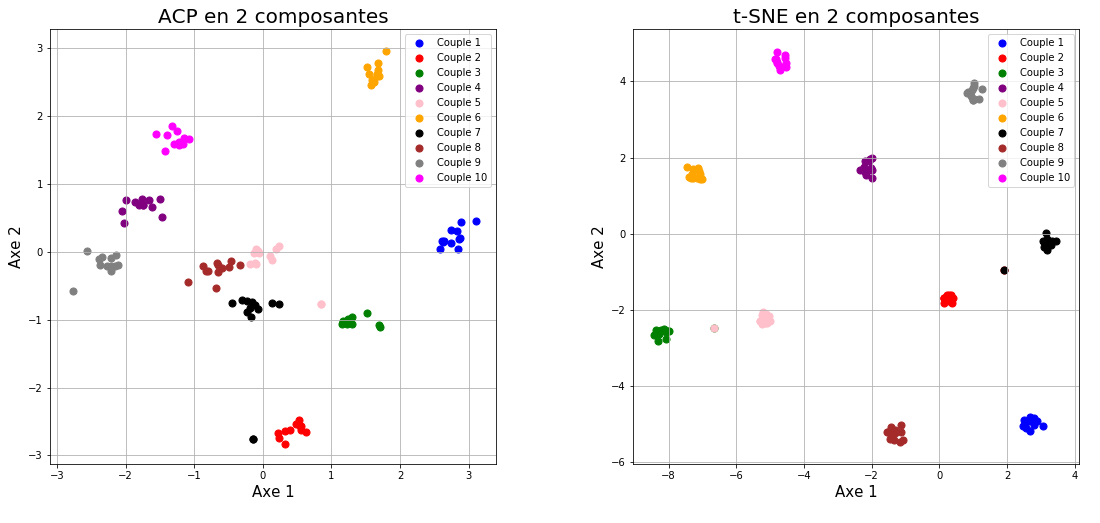
\includegraphics[width=1\textwidth]{figures.png}
\captionsetup{margin=0cm,format=hang,justification=justified}
\caption{Évaluation du modèle sur données fictives}\label{fig:figure_evaluation}
\end{figure}

Quelle que soit la problématique choisie à terme, nous tenterons de
calculer des indicateurs synthétiques à l'aide de techniques d'analyse
de sentiments. Nous devons également garder en tête les différentes
limites des données à notre disposition : leur faible profondeur
temporelle rendant complexe la prévision de données trimestrielles ou
encore leur thématique se rapprochant certainement davantage des
questions d'opinions des ménages plutôt que des informations liées aux
entreprises.

\nocite{*}

\begin{thebibliography}{999}
\bibitem[Bortoli, C., Combes, S., Renault, T. (2018)]{Monde} Bortoli, C., Combes, S., Renault, T. (2018). Nowcasting GDP Growth by Reading Newspapers. Economie et Statistique / Economics and Statistics, 505-506, 17–33. \url{https://doi.org/10.24187/ecostat.2018.505d.1964 }.
\bibitem[Mikolov, T., et al. (2013)]{Mikolov}Mikolov, T.,  Chen, K., Corrado, G., Dean, J. (2013). Efficient Estimation of Word Representations in Vector Space \url{https://arxiv.org/pdf/1301.3781.pdf}.
\bibitem[Srivastava, M., Nguyen, T. (2018)]{Chomage}Srivastava, M., Nguyen, T. (2018). “Nowcasting” County Unemployment Using Twitter Data. \url{https://web.stanford.edu/class/archive/cs/cs224n/cs224n.1174/reports/2737035.pdf}.
\end{thebibliography}

\end{document}